\documentclass[11pt]{beamer}
\usetheme{Bergen}
\usepackage[utf8]{inputenc}
\usepackage{amsmath}
\usepackage{amsfonts}
\usepackage{amssymb}
\usepackage{graphicx}
\usepackage{hyperref}
\usepackage{fontawesome}
\usepackage{xcolor}
\usepackage{movie15}
\usepackage{dsfont}
\usepackage{tikz}
\def\insertauthorindicator{Ponente}
\def\insertinstituteindicator{Instituto}
\def\insertdateindicator{Fecha}
\usetikzlibrary{decorations.markings}

\tikzset{
  invisible/.style={opacity=0},
  visible on/.style={alt={#1{}{invisible}}},
  alt/.code args={<#1>#2#3}{%
    \alt<#1>{\pgfkeysalso{#2}}{\pgfkeysalso{#3}} % \pgfkeysalso doesn't change the path
  },
}
\setbeamertemplate{footline}[frame number]
\author{José Antonio García Hernández}
\title{Métodos Monte Carlo en Teorías Cuánticas de Campos (Lattice QFT)}
\setbeamercovered{transparent} 
\setbeamertemplate{navigation symbols}{} 

\institute{Instituto de Ciencias Nucleares, UNAM} 
\date{29 noviembre 2024 \\ XX Congreso de Estudiantes del PCF} 
\subject{Lattice Field Theories} 
\begin{document}

\begin{frame}
\titlepage

\includegraphics[width=3cm]{icn.png}
\end{frame}

%\begin{frame}
%\tableofcontents
%\end{frame}

\section{Introducción}
\subsection{Integral funcional}
\begin{frame}{Formalismo de la integral funcional}

    Integral funcional: Suma sobre todas  las configuraciones del campo $\phi(x)$
    $$Z = \int \mathcal{D}\phi \, e^{iS[\phi]},$$
    donde $S[\phi]$ es la acción% de la configuración
    $$ S[\phi] = \int d^4 x \, \left( \frac{1}{2}\partial_{\mu}\phi \partial^{\mu}\phi - V(\phi)\right).$$
    Funciones de $n$ puntos
    $$ \langle O[\phi(x_1)] \cdots \rangle =  \frac{1}{Z}\int \mathcal{D}\phi \, O[\phi(x_1)]\cdots e^{iS[\phi]}.$$
\end{frame}

\begin{frame}{Rotación de Wick. Espacio euclidiano}
    Rotación de Wick \\~
    $$ t \to \tau = i t.$$
    %Espaciotiempo de Minkowski $\to$ Espaciotiempo euclidiano \\~
    $$ \eta_{\mu\nu} \to \delta_{\mu\nu}$$
        
    Factor de peso 
        $$ \int \mathcal{D}\phi \, e^{iS[\phi]} \to  \int \mathcal{D}\phi \, e^{-S_{\text{E}}[\phi]},$$
        donde 
        $$ S_{\text{E}}[\phi] = \int d^4 x \, \left( \frac{1}{2}\partial_{\mu}\phi \partial_{\mu}\phi + V(\phi)\right).$$
        Función de partición $ Z = \int \mathcal{D}\phi\, e^{-\beta H[\phi]}$.
        
        Teoría de campos $\to$ Física estadística. 
\end{frame}

\subsection{Regularización de la retícula}
\begin{frame}{Regularización de la retícula (Lattice Regularization).}
    Divergencias ultravioleta.\\~
    
    Regularización de la retícula: %Discretizar el espaciotiempo
    
    \begin{center}
    \begin{tikzpicture}[scale = 0.5]
    	\draw (-0.5,-0.5) grid (2.5,2.5);
    	\fill[red] (1,1) circle(0.15);
    	\draw[red] (1.5,1.5) node[]{$\phi_x$};
    	\draw[blue] (2,0) node[above right]{ $a$};
    	\draw[-latex, thick] (4,1) --(4,2) node[left]{\small $\hat{2}$};
	\draw[-latex, thick] (4,1) --(5,1) node[right]{\small $\hat{1}$};
    \end{tikzpicture}
    \end{center}
    \begin{itemize}
    		\item $\phi(x) \to \phi_x$
         \item $\displaystyle\partial_\mu\phi(x) \to \frac{\phi_{x + a\hat{\mu}} - \phi_x}{a}$
         \item $\displaystyle\int d^4x \to a^4\sum_{x}$
    \end{itemize}
    
    Unidades de lattice $a = 1$. \\~
    
    Formalismo NO PERTURBATIVO.
\end{frame}

\begin{frame}{Cadenas de Markov}

    Generamos una cadena de configuraciones donde la configuración actual depende solo de la anterior (cadena de Markov)
    
    $$ [\phi_1] \to [\phi_2] \to \cdots$$

    $$\langle O \rangle = \frac{1}{N}\sum_{i=1}^N O[\phi_i]$$
    donde $[\phi_i]$ es generada con probabilidad $\frac{1}{Z}e^{-S_{\text{E}}[\phi_i]}$.
\end{frame}

\begin{frame}{Muestreo de importancia (importance sampling)}
    Para generar configuraciones, el algoritmo necesita cumplir
    \begin{itemize}
        \item<1-> Ergodicidad
        \begin{center}
        		\begin{tikzpicture}
        			\draw (0,0) rectangle (4,2);
        			\draw[blue] (0.1,0.5) -- (1,1.18) -- (3, 0.3) -- (3.7, 1.9) -- (1, 0.1) --(0.8,1.8) -- (2,1.5);
        		\end{tikzpicture}
        \end{center}
        \item<2-> Balance detallado (detailed balance)
        \begin{center}
        \begin{tikzpicture}
    		\coordinate (A) at (0.7,0.7);
    		\coordinate (B) at (3,1.5);
    		\draw (0,0) rectangle (4,2);
    		\fill[] (A) circle(0.1) node[left]{$A$};
    		\fill[] (B) circle(0.1) node[right]{$B$};
    		\draw[blue,thick, -latex] (A) to[out = 90, in = 180] (B);
    	\draw[red,thick, -latex] (B) to[out = -90, in = 0] (A);		
    		
    \end{tikzpicture}
    \end{center}
    $$ p[A]p[A \to B] = p[B]p[B \to A]$$
    \end{itemize}
    
    
\end{frame}

\begin{frame}{Algoritmos de actualización}
    Locales
    \begin{itemize}
        \item Metropolis
        \item Glauber
        \item Heatbath
        %\item Hybrid Monte Carlo
        \item etc\dots
    \end{itemize}
    
    \ \\~
    
    Globales
    \begin{itemize}
        \item Wolff
        \item Swendsen-Wang
    \end{itemize}
\end{frame}

\begin{frame}{Algoritmo Metropolis}
    \begin{itemize}
        \item Escogemos un sitio $x$ de la retícula.
        \item Generamos una propuesta del campo a actualizar $\phi_x \to \phi'_x$.
        \item Aceptamos la propuesta con probabilidad 
        $$ p = \min\left(1, \exp\left(-\Delta S\right)\right),$$
           donde
        $$ \Delta S = S[\phi'] - S[\phi].$$        
        %(Generamos un número aleatorio $r\in[0,1)$ si $r<p$, $\phi_x$ se actualiza a $\phi'_x$. Si $r>p$, rechazamos el cambio y conservamos a $\phi_x$.)
      
      	\item Aplicamos los pasos anteriores a todos los puntos de la retícula (\emph{sweep}). 
    \end{itemize}
\end{frame}

\begin{frame}{Simulación Monte Carlo}

    \begin{itemize}
    		\item Configuración inicial \emph{\textcolor{red}{hot}} o \emph{\textcolor{blue}{cold}} \emph{start}.
        \item Generación de configuraciones.
        \item Equilibrio.
        \item Toma de mediciones.
        \item Cálculo de promedios y errores (comúnmente \emph{jackknife}).
        \item Interpretación de resultados.
    \end{itemize}

\end{frame}

\section{Ejemplos}
\subsection{Modelo de Ising}
\begin{frame}{Ejemplo: Modelo de Ising 2d}

Espín clásico $s_x\in\{-1,1\}$. \\~

Función hamiltoniana
$$ H[s] = -J\sum_{\langle xy \rangle} s_x s_y,$$
$x$, $y$ son puntos en la retícula y $\langle xy \rangle$ representa la suma sobre primeros vecinos.\\~

Función de partición
$$ Z = \sum_s e^{-\beta H[s]}.$$

Definimos
$$S[s] = \beta H[s].$$

\end{frame}

\begin{frame}{Paso Metropolis}
\begin{tikzpicture}
	\coordinate (A) at (0,0.5);
	\coordinate (B) at (0,-0.5); 
	\draw (-0.5,-0.5) grid (3.5,3.5);
	\draw[-latex, very thick] (4,2.5) --(4,3.5) node[left]{$\hat{2}$};
	\draw[-latex, very thick] (4,2.5) --(5,2.5) node[right]{$\hat{1}$};
	\draw[visible on = <1>] (6,2) node[]{Configuración de espines $[s]$};
	\draw[visible on = <1>] (6,1) node[]{Fijamos $\beta = \frac{1}{4}$.};
	\draw[-latex,very thick,blue, visible on=<1->] (0,0) -- +(A);
	\draw[-latex,very thick,red, visible on=<1->]  (1,0) -- +(B);
	\draw[-latex,very thick,blue,visible on=<1->] (2,0) -- +(A);
	\draw[-latex,very thick,blue,visible on=<1->] (3,0) -- +(A);
	\draw[-latex,very thick,red,visible on=<1->]  (0,1) -- +(B);
	\draw[-latex,very thick,red,visible on=<1-11>] (1,1) -- +(B);
	\draw[-latex,very thick,red,visible on=<1->]  (2,1) -- +(B);
	\draw[-latex,very thick,red,visible on=<1->]  (3,1) -- +(B);
	\draw[-latex,very thick,blue,visible on=<1->] (0,2) -- +(A);
	\draw[-latex,very thick,blue,visible on=<1->] (1,2) -- +(A);
	\draw[-latex,very thick,blue,visible on=<1->] (2,2) -- +(A);
	\draw[-latex,very thick,red,visible on=<1->]  (3,2) -- +(B);
	\draw[-latex,very thick,red,visible on=<1->]  (0,3) -- +(B);
	\draw[-latex,very thick,blue,visible on=<1->] (1,3) -- +(A);
	\draw[-latex,very thick,red,visible on=<1->]  (2,3) -- +(B);
	\draw[-latex,very thick,blue,visible on=<1->] (3,3) -- +(A);
	
	\draw[red,visible on=<2-11>] (0.5,0.5) node[right]{$s_x$};
	\draw[visible on = <2>] (6,2) node[]{Escogemos un sitio $x$};
	
	\draw[visible on = <3>] (6,2) node[]{Proponemos $s_x \to s'_x$};
	\draw[-latex,very thick,blue,opacity=1,visible on =<3->]  (1,1) -- +(A);
	\draw[blue,dashed,visible on=<3-11>] (1,1.3)  circle(0.3);
	\draw[blue,visible on=<3-11>] (1.5,1.5) node[]{$s'_x$};
	
	\draw[visible on = <4-6>] (6,2) node[]{Calculamos $\Delta S $};
	\draw[visible on = <5-6>] (4,-1) node[]{$\Delta S = 2\beta s_x\cdot(s_{x+\hat{1}} + s_{x-\hat{1}} + s_{x+\hat{2}} + s_{x-\hat{2}})$};
	
	\draw[visible on = <6>] (4,-2) node[]{$\Delta S = 2(\frac{1}{4})(-1)(-1-1-1+1) = 1$};
	
	\draw[visible on = <7>] (4,-1) node[]{Aceptamos el cambio con probabilidad};
	\draw[visible on = <7>] (4,-2) node[]{$p = \min(1,e^{-\Delta S}) = \min\left(1,e^{-1}\right) = e^{-1}\approx 0.37$};
	
	\draw[visible on = <8-11>] (4,-1) node[]{$p \approx 0.37$};
	\draw[visible on = <8-11>] (4,-2) node[]{Generamos un número aleatorio $r \in[0,1)$};
	\draw[visible on = <9>] (4,-3) node[]{$r = 0.1375\dots$};
		\draw[visible on = <10-11>] (4,-3) node[]{$r = 0.1375\dots < p = 0.37$};
		\draw[visible on = <11>] (4,-4) node[]{Aceptamos el cambio $\checkmark$};
		
		\draw[visible on = <12>] (4,-2) node[]{Nueva configuración};
\end{tikzpicture}
\end{frame}

\begin{frame}{Termalización}
%    \includemovie[autoplay]{\textwidth}{\textwidth}{figures/ising.mp4}
\end{frame}

\subsection{Oscilador anarmónico cuántico}
\begin{frame}{Ejemplo: Oscilador anarmónico cuántico 1d}

    Lagrangiano euclidiano

    $$ L_{\text{E}} = \frac{1}{2}m\left(\partial_{\tau}x\right)^2 + \frac{1}{2}m\omega^2 x^2 + \lambda x^4,$$
con $\lambda \ge 0$. \\~

Del teorema del virial 
$$\langle T \rangle = \frac{1}{2}\langle x V'(x) \rangle$$
calculamos la energía del estado base $E_0$ 
$$ E_0 = m\omega^2\langle x^2 \rangle + 3\lambda \langle x^4 \rangle. $$
\end{frame}

\begin{frame}{Oscilador armónico}
    %\includemovie[autoplay]{\textwidth}{\textwidth}{figures/harmonic_oscillator_path.mp4}
\end{frame}

\begin{frame}{Oscilador anarmónico}
    %\includemovie[autoplay]{\textwidth}{\textwidth}{figures/anharmonic_oscillator_path.mp4}
\end{frame}

\subsection{Teoría $\lambda \phi^4$}
\begin{frame}{Ejemplo: Teoría $\lambda \phi^4$ 2d}

Sea un campo escalar $\phi(t,x)\in\mathbb{R}$.\\~

Densidad lagrangiana euclidiana

    $$ \mathcal{L}_{\text{E}} = \frac{1}{2}\partial_{\mu} \phi \partial_{\mu}\phi + \frac{1}{2}m^2  \phi^2 + \frac{\lambda}{4} \phi^4,$$
    con $\lambda \ge 0$. \\~
    
	Función de 2 puntos
	$$ \langle \phi(t,x)\phi(t + \tau,x)  \rangle \propto \exp(-m_r \tau).$$    
    
\end{frame}

\begin{frame}{Fase simétrica}
    %\includemovie[autoplay]{\textwidth}{\textwidth}{figures/symmetric_phase_evolutionfield.mp4}
\end{frame}

\begin{frame}{Fase rota}
    %\includemovie[autoplay]{\textwidth}{\textwidth}{figures/broken_phase_evolutionfield.mp4}
\end{frame}

\begin{frame}{Función de correlación}
Con $\lambda = 0.05$ y $m^2 = -0.75$ 
\begin{center}
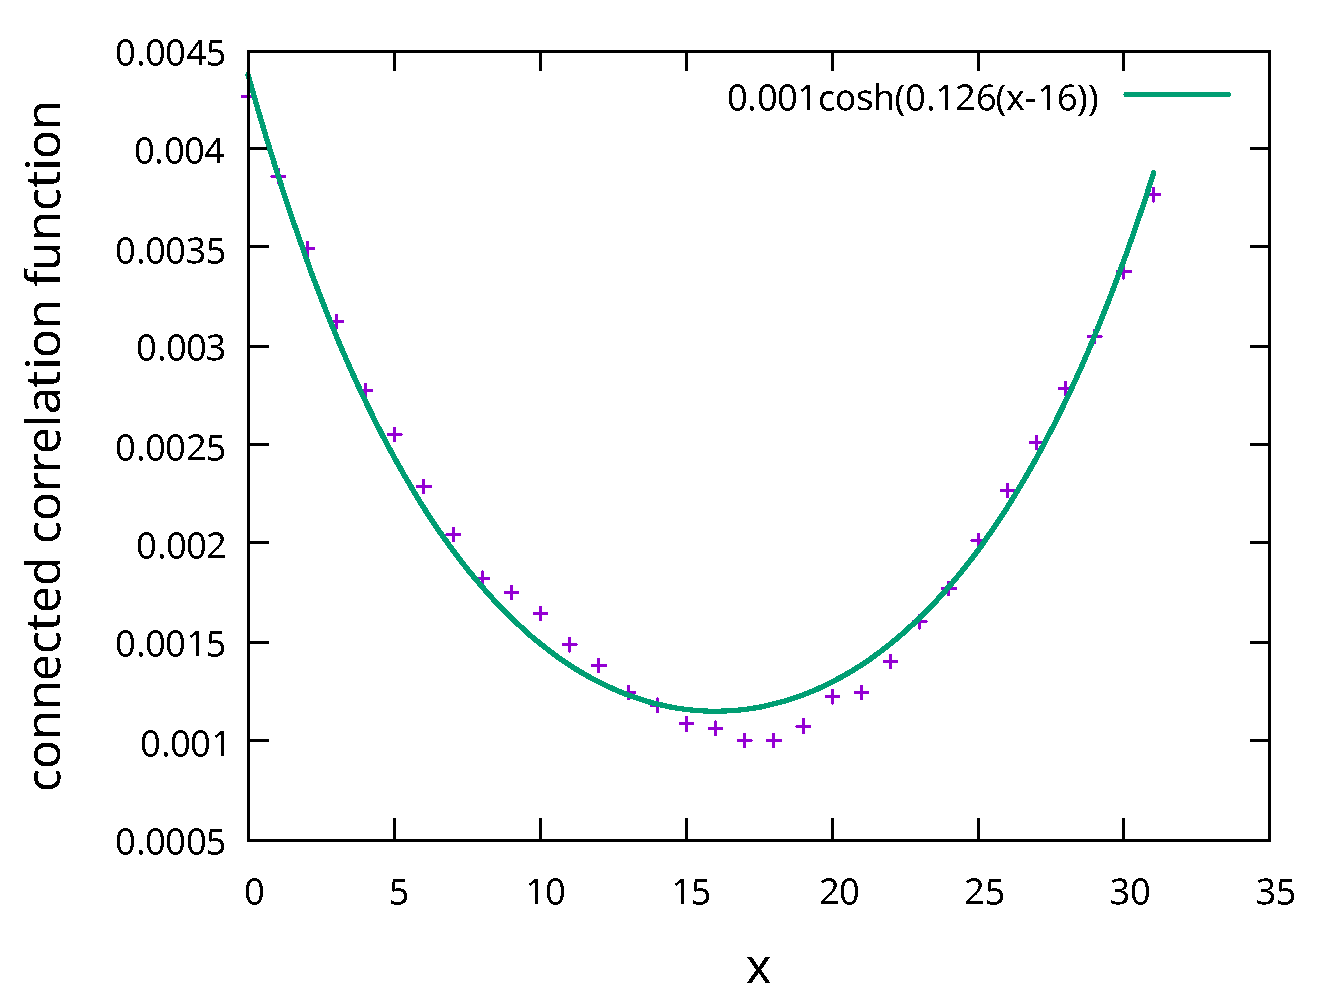
\includegraphics[scale=0.3]{figures/correlation_function.pdf}
\end{center}

$$ m_r = 0.1120(8). $$
\end{frame}

\begin{frame}{Teoría de norma en la retícula}


Formulación compacta 
$$A_{\mu}(x) \in \mathfrak{su}(N) \to U_{\mu}(x) \in \text{SU}(N), \ \ \ U_{\mu}(x) = e^{iA_{\mu}(x)}$$ 

	\begin{tikzpicture}[scale = 0.7]
		\tikzset{middlearrow/.style={decoration={markings,mark= at position 0.6 with {\arrow{#1}} ,},postaction={decorate}}};
		\draw[step=2cm,color=gray] (-1,-1) grid (3,3);
		\draw[middlearrow={latex}, very thick,red] (0,0) --(2,0);
		\draw[middlearrow={latex}, very thick,red] (2,0)--(2,2);
		\draw[middlearrow={latex}, very thick,red] (2,2)--(0,2);
		\draw[middlearrow={latex}, very thick,red] (0,2)--(0,0);
		\filldraw[black] (0,0) circle(0.1);
		\filldraw[black] (2,0) circle(0.1);
		\filldraw[black] (2,2) circle(0.1);
		\filldraw[black] (0,2) circle(0.1);
		\draw[] (0,0) node[below left] {\tiny  $x$};
		\draw[] (2,0) node[below right] {\tiny  $x+\hat\mu$};
		\draw[] (0,2) node[above left] {\tiny  $x+\hat\nu$};
		\draw[] (2,2) node[above right] {\tiny  $x+\hat\mu+\hat\nu$};
		
		\draw[] (8,1) node[] {\small  $U_{x,\mu\nu} = U^{\dagger}_{x,\nu} U^{\dagger}_{x+\hat\nu,\mu}U_{x+\hat\mu,\nu}U_{x,\mu}$};
		
		\draw[blue] (1,0) node[below] {\small $U_{x,\mu}$};
		\draw[blue] (2,1) node[right] {\small  $U_{x+\hat\mu,\nu}$};	
		\draw[blue] (1,2) node[above] {\small  $U^{\dagger}_{x+\hat\nu,\mu}$};
		\draw[blue] (0,1) node[left] {\small  $U^{\dagger}_{x,\nu}$};
			
	\end{tikzpicture}
     
    Acción estándar de Wilson
$$ S[U] = \frac{\beta}{N}\sum_{x}\sum_{\mu < \nu} \text{Tr Re} \left[\mathds{1} - U_{x,\mu\nu} \right], $$
donde $\beta = 2N/g^2$, con $g$ el acoplamiento de norma. 

\end{frame}

%\subsection{Teoría de norma U(1)}
%\begin{frame}{Ejemplo: Teoría de norma U(1) 2d}
%
%Acción estándar de Wilson
%$$ S[U] = \beta\sum_{x}\sum_{\mu < \nu} \text{Re} \left[1 - U_{\mu\nu} \right], $$
%donde $\beta = 2/g^2$, con $g$ el acoplamiento de norma. 
%\end{frame}
%
%\begin{frame}
%\begin{center}
%
%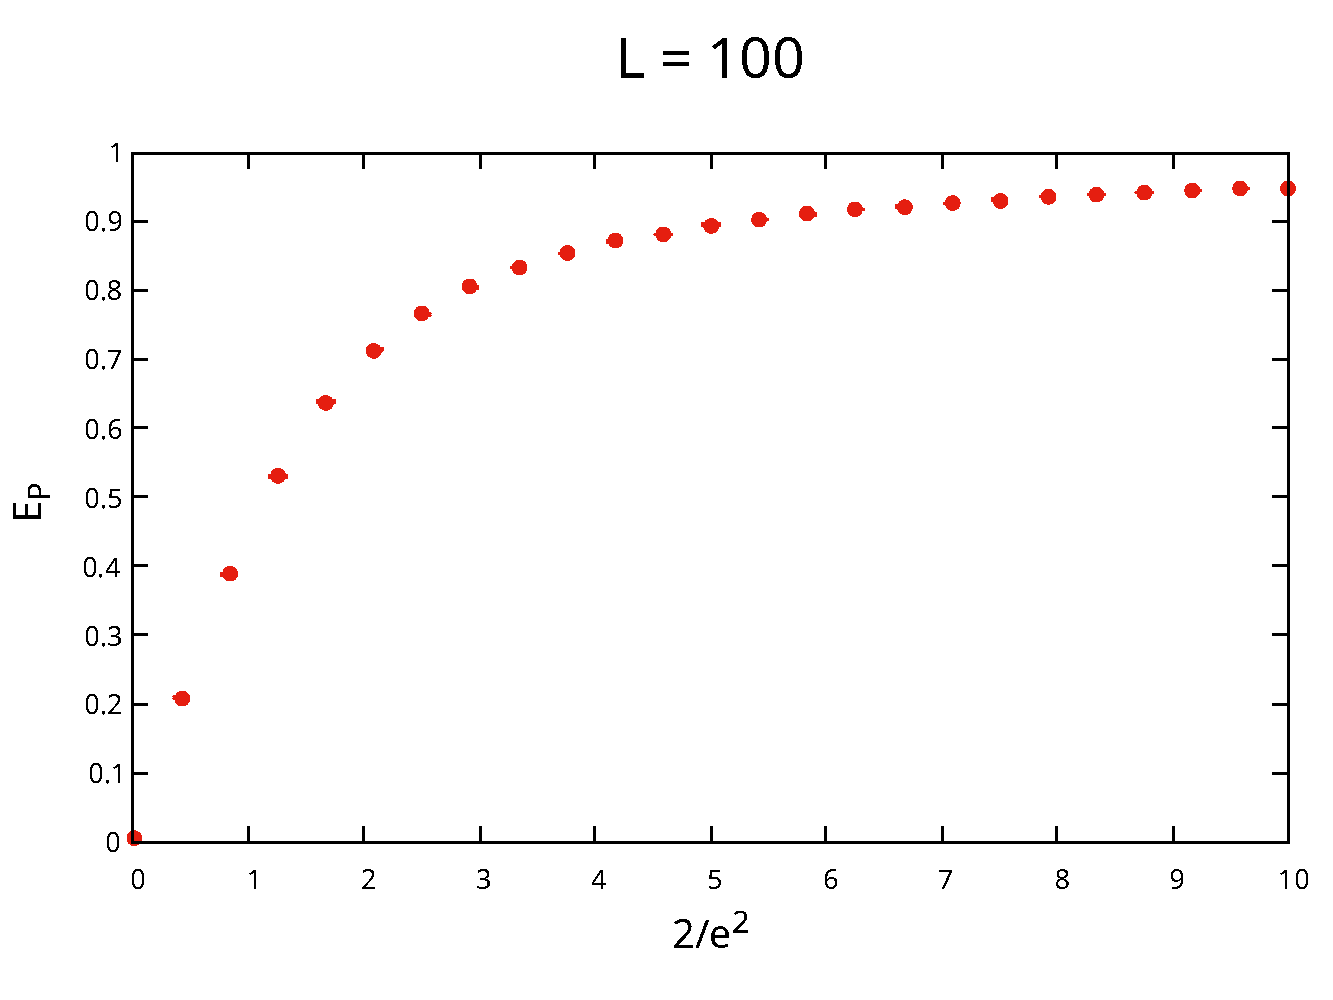
\includegraphics[scale=0.3]{figures/L100.pdf}
%\end{center}
%\end{frame}


%\subsection{Teoría de norma SU(2)}
%\begin{frame}{Ejemplo: Teoría de norma SU(2) 4d}
%Acción estándar de Wilson
%$$ S[U] = \frac{\beta}{2}\sum_{x}\sum_{\mu < \nu} \text{Re Tr} \left[\mathds{1} - U_{\mu\nu} \right] $$
%\end{frame}
%
%\begin{frame}
%\begin{center}
%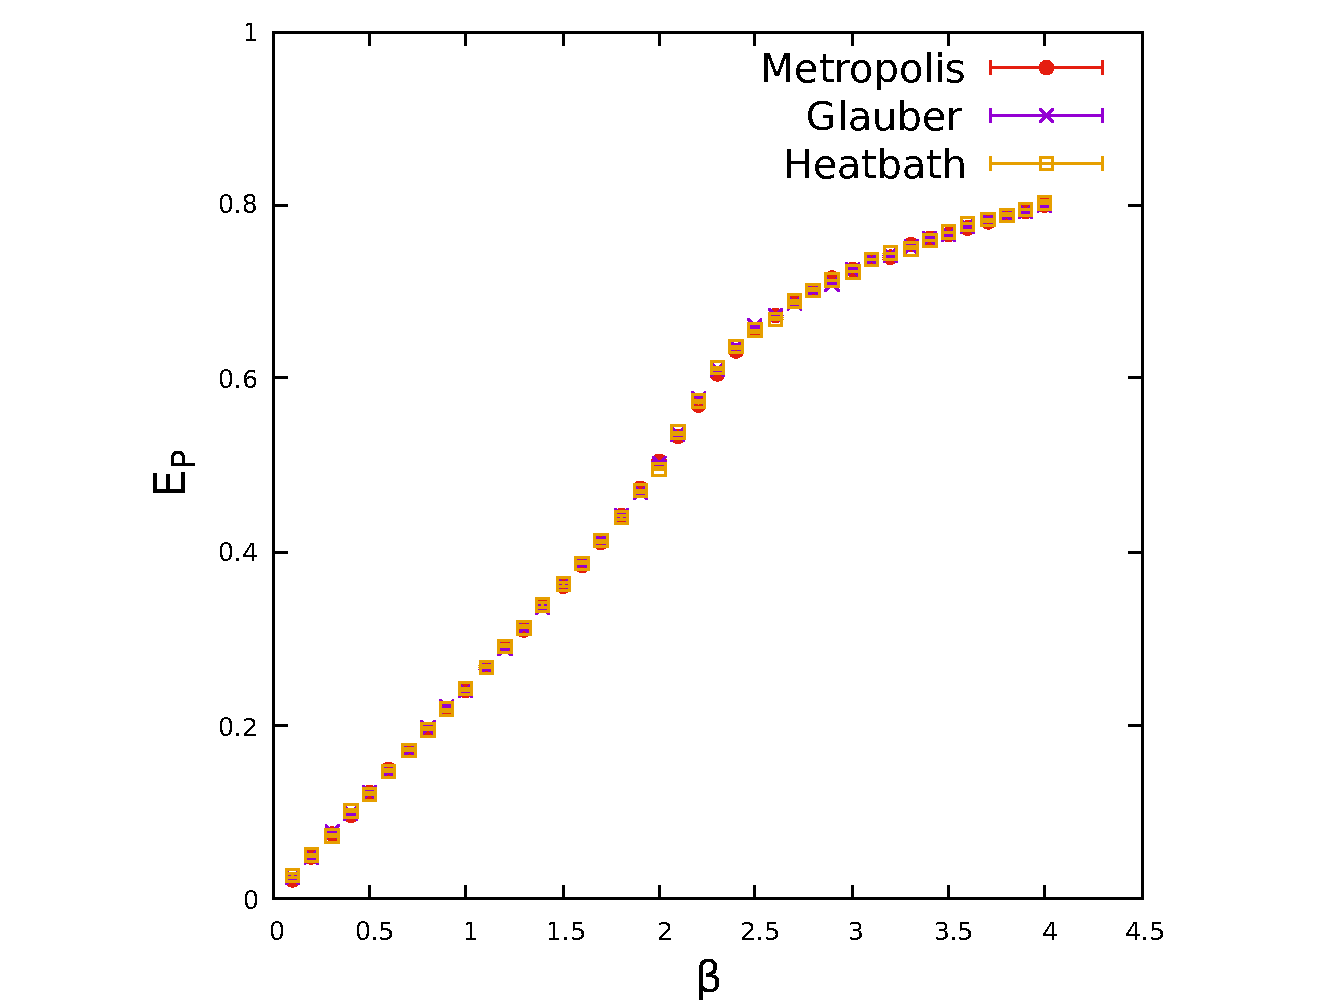
\includegraphics[scale=0.3]{figures/L=4_metropolis_glauber_heatbath.pdf}
%\end{center}
%\end{frame}
%
%\begin{frame}
%\begin{center}
%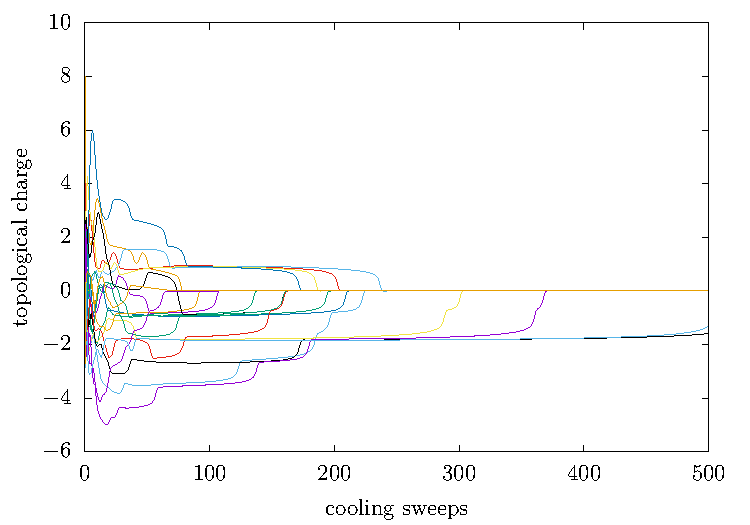
\includegraphics[scale=0.6]{figures/cooling.pdf}
%\end{center}
%\end{frame}

\subsection{Teoría de norma SU(3)}
\begin{frame}{Ejemplo: Teoría de norma SU(3) 4d}
Acción estándard de Wilson
$$ S[U] = \frac{\beta}{3}\sum_{x}\sum_{\mu < \nu} \text{Re Tr} \left[\mathds{1} - U_{\mu\nu} \right].$$

Loop de Polyakov
$$ P(\vec{x}\,) = \text{Tr}\,\prod_{t_\text{E}=1}^{L_t}U_4(\vec{x},t_\text{E}).$$
\end{frame}

\begin{frame}{Valor de la plaqueta}
\begin{center}
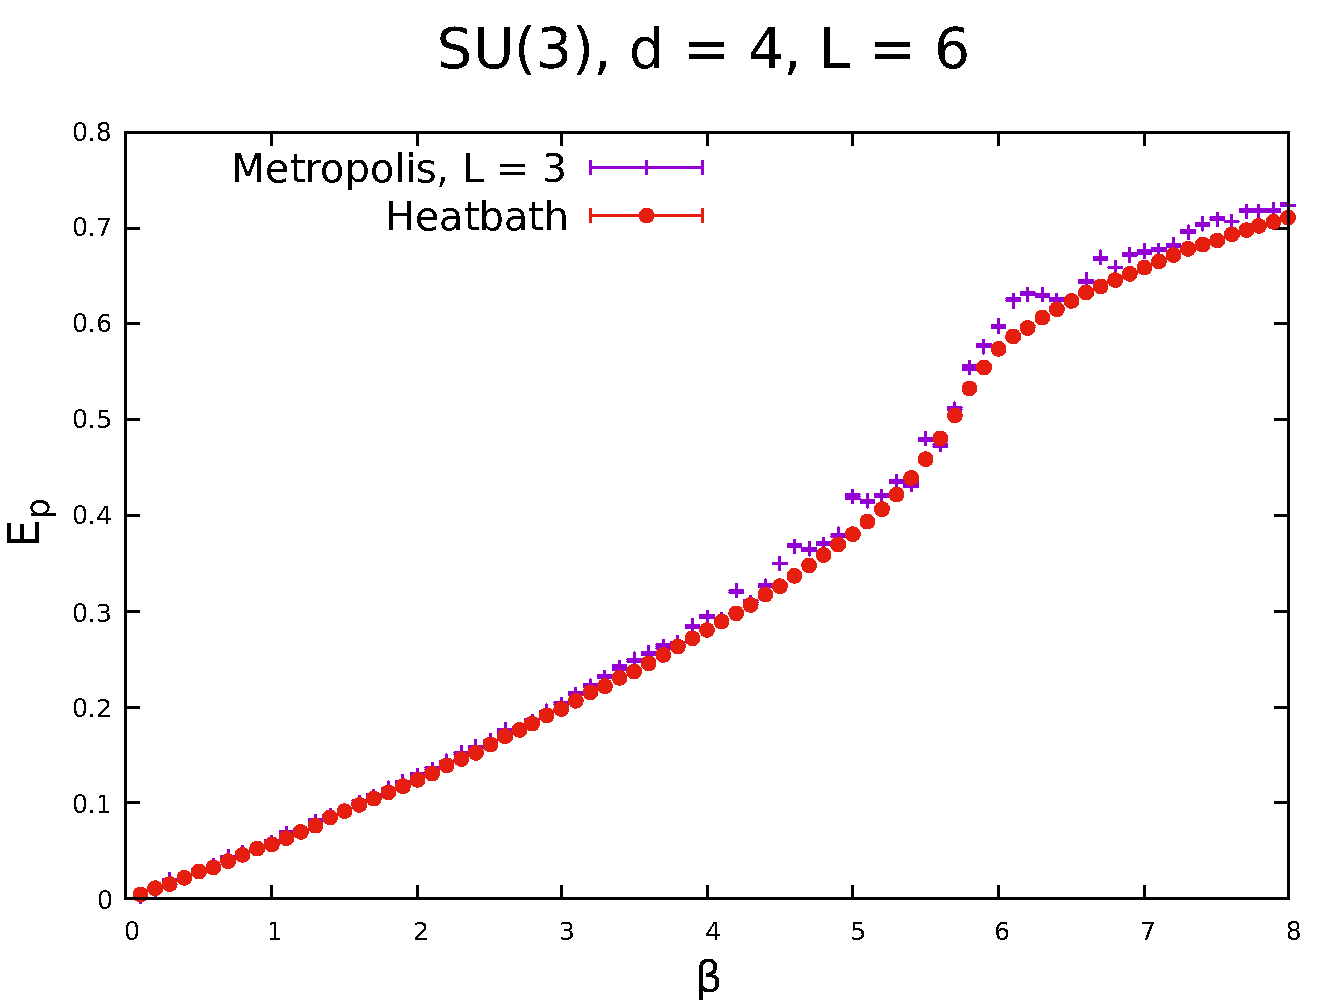
\includegraphics[scale=0.3]{figures/L=6_heatbath_L=3_metropolis.pdf}
\end{center}
\end{frame}

\begin{frame}{Rompimiento espontáneo de $Z_3$}
%\begin{center}
\begin{minipage}[l]{0.5\textwidth}
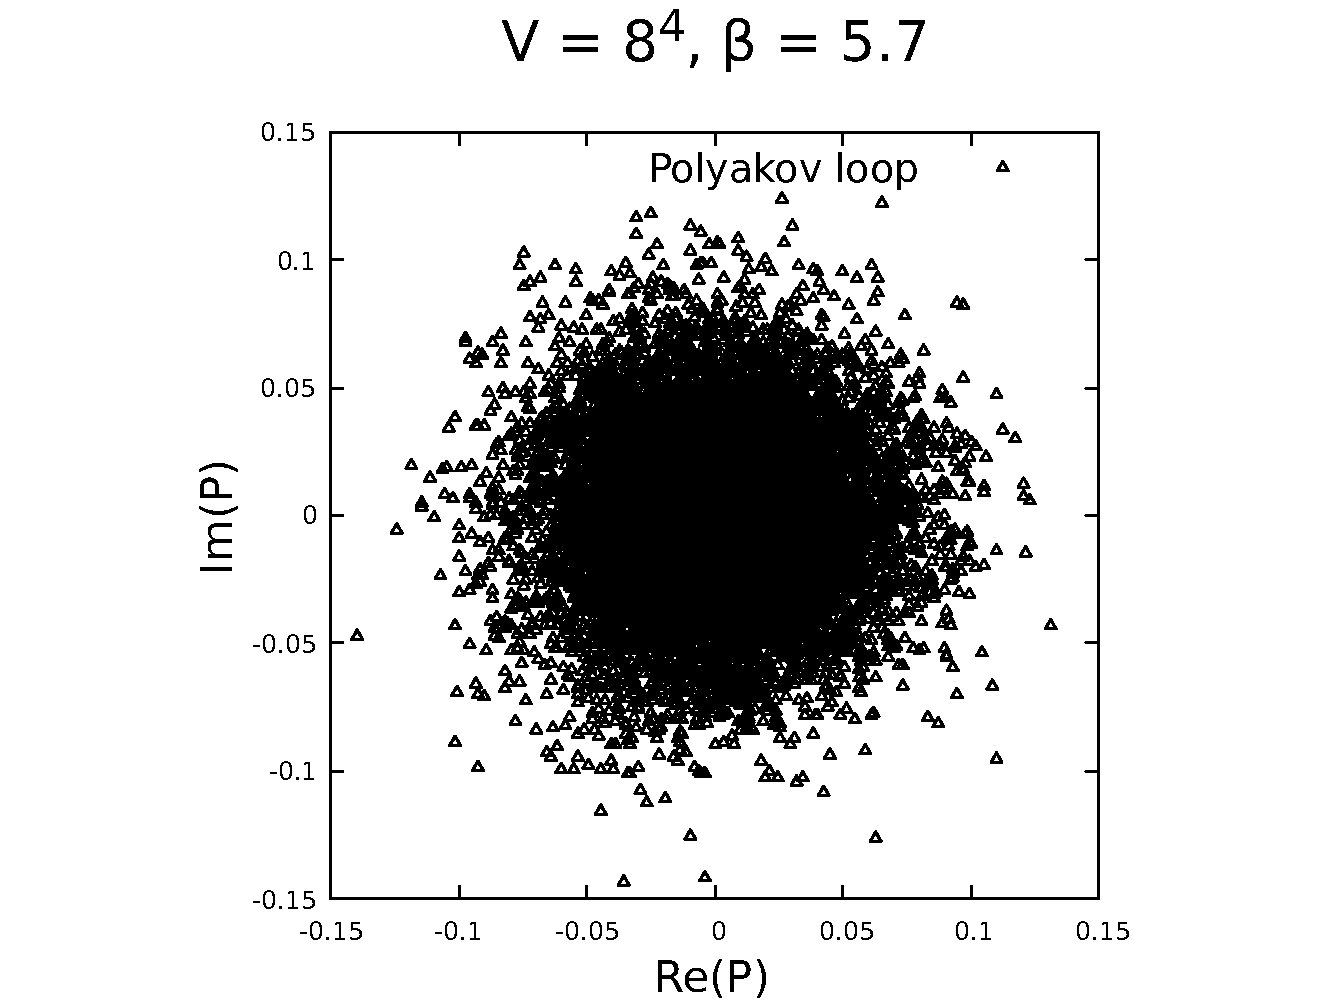
\includegraphics[scale=0.2]{figures/polyakov_loop_beta=5_7.pdf}
\end{minipage}\begin{minipage}[l]{0.5\textwidth}
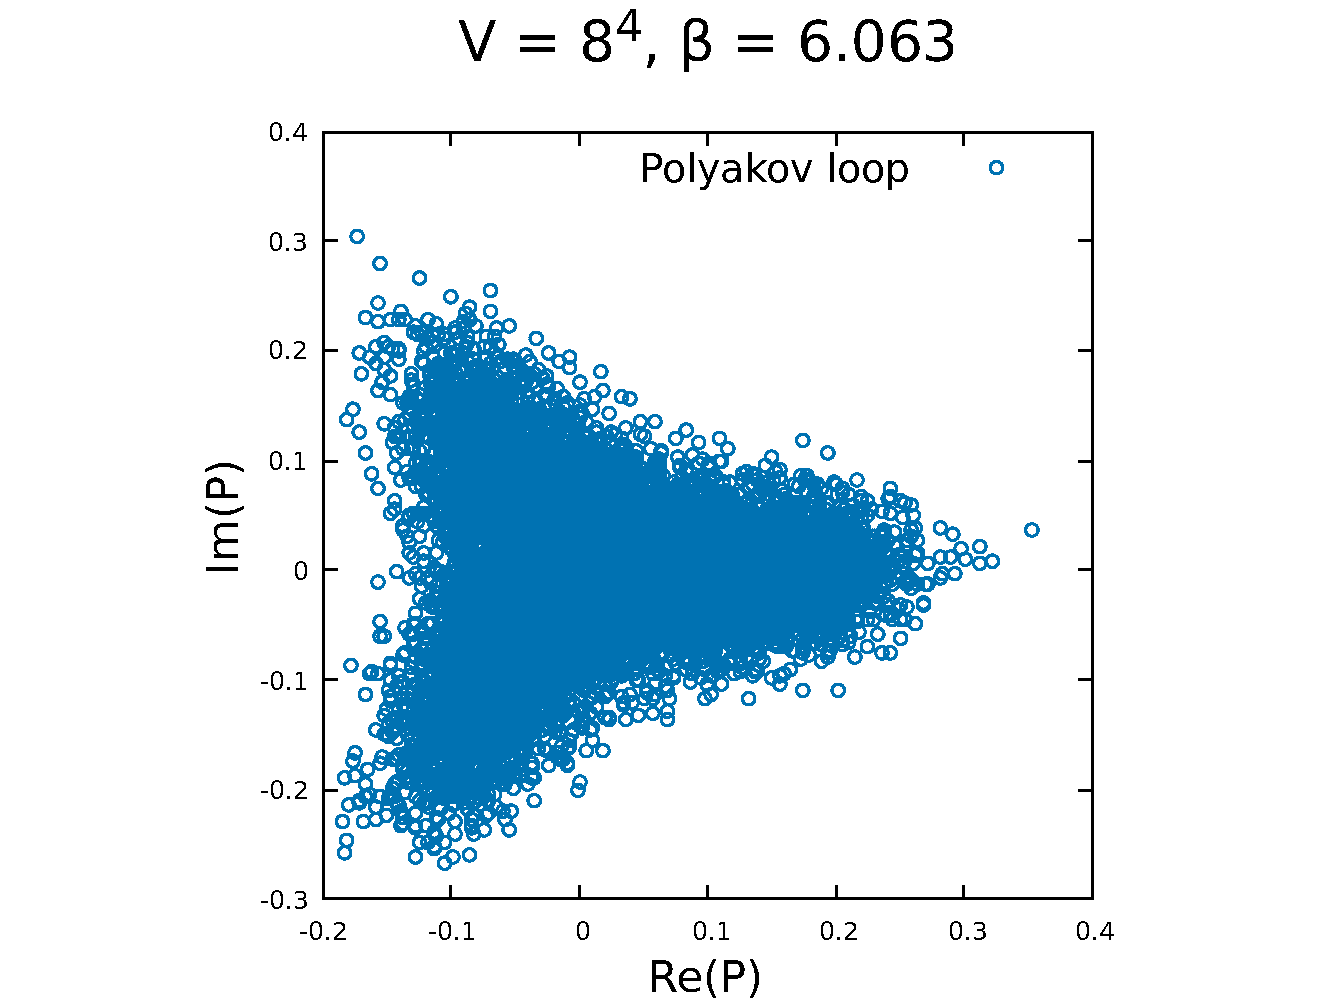
\includegraphics[scale=0.2]{figures/polyakov_loop.pdf}
\end{minipage}

%\end{center}
\end{frame}

\section{Resumen}
\begin{frame}{Resumen}

Formalismo de la integral funcional, método alternativo a cuantización canónica. \\~

Rotación de Wick: QFT $\to$ Fís.\ Estadística.  \\~

Regularización de \emph{lattice} es un enfoque no perturbativo e invariante de norma. \\~

Formulación compacta para teorías de norma NO requiere fijar la norma. \\~

La formulación de \emph{lattice} es muy ROBUSTA.\\~

¡Colaboradores BIENVENIDOS!
    
\end{frame}

\begin{frame}{Referencias}

¡Siganme en mi GitHub \faGithub !
\url{https://github.com/JoseAntonioLattice}
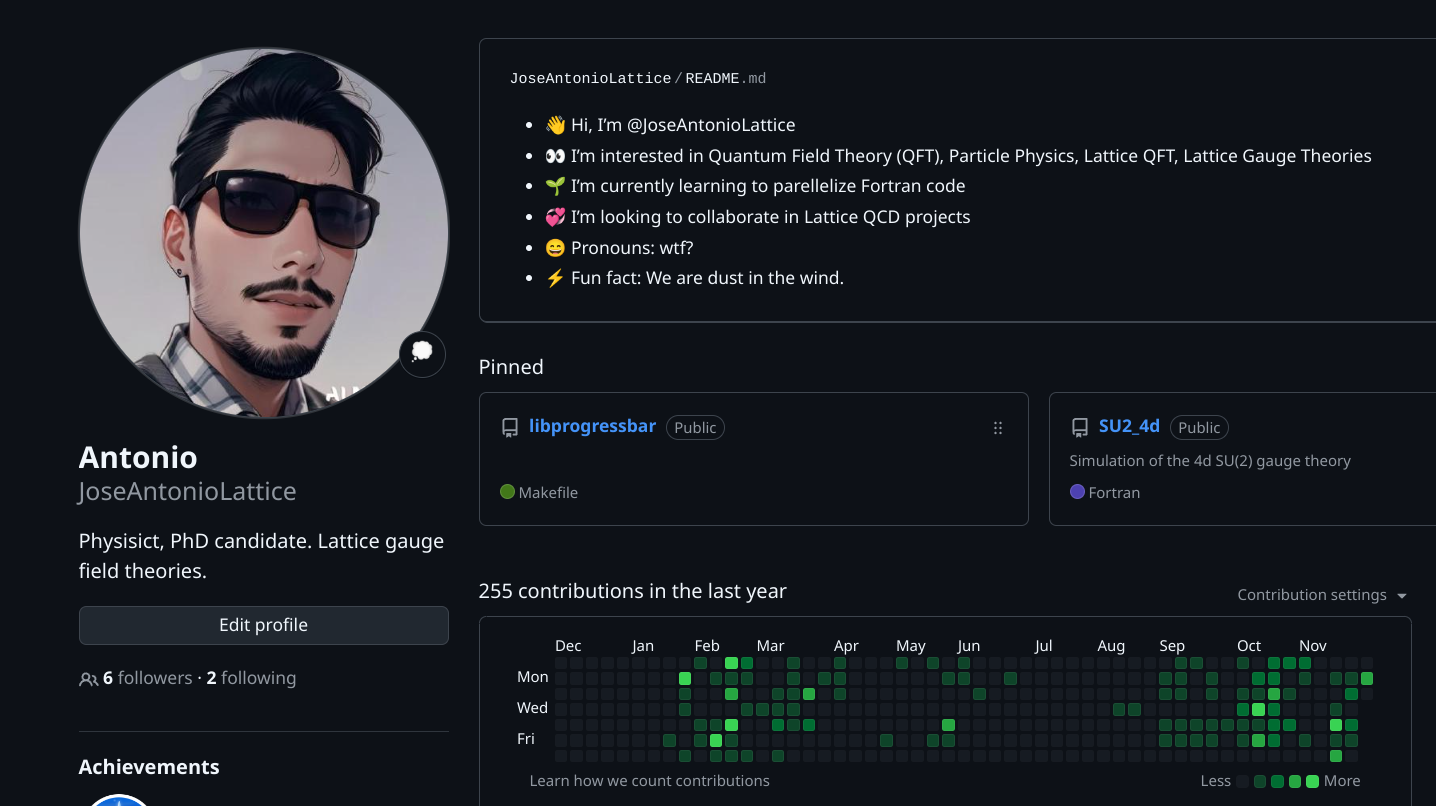
\includegraphics[scale=0.15]{figures/github.png}
\end{frame}


\end{document}
